\section{Ejercicio 5}

Este ejercicio es similar al anterior y lo que se quiere ver es como evoluciona la loss y el accuracy cuando se tienen las funciones de activación RELU en la primera capa y Sigmoide o Lineal para la segunda.
El grafo computacional correspondiente a este problema es el que se muestra en la siguiente figura:

\begin{figure}[H]
    \centering
    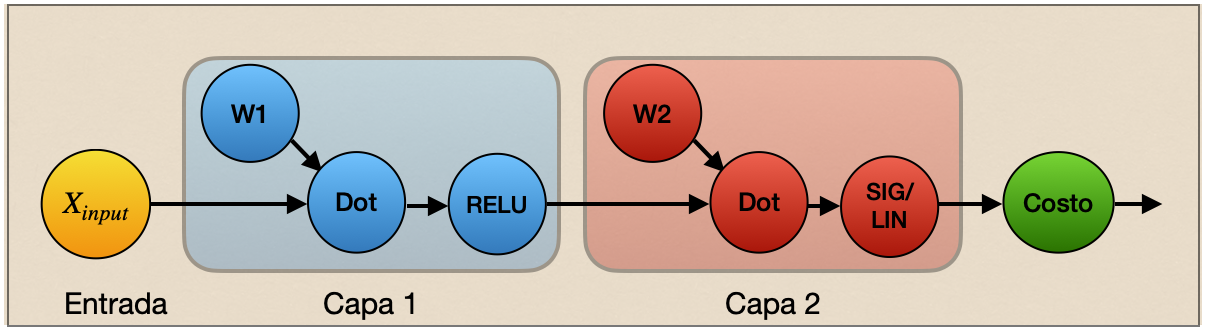
\includegraphics[height=1.5in]{image/EJ5.png}
    \caption{Grafo computacional del Ejercicio 5}
    \label{fig:ej5}
\end{figure}

Para la primera combinación RELU+Sigmoide utilizando como hiperparámetros:
\begin{verbatim}
nclases = 10  # Cantidad de neuronas de la 2º capa
nintermedia = 100  # Cantidad de neuronas de la 1º capa
batch_size = 128  # Tamaño del Batch
n_epocas = 50  # Cantidad de épocas para entrenar
learning_rate = 1e-6  # Tasa de aprendizaje
reg_lambda = 0.1  # Factor de regularización
n_train_data = 10000  # Cantidad de datos utilizados para el entrenamiento de la red
\end{verbatim}  
se obtuvieron las siguiente gráficas:

\begin{figure}[H]
     \centering
     \begin{subfigure}[b]{0.45\textwidth}
         \centering
         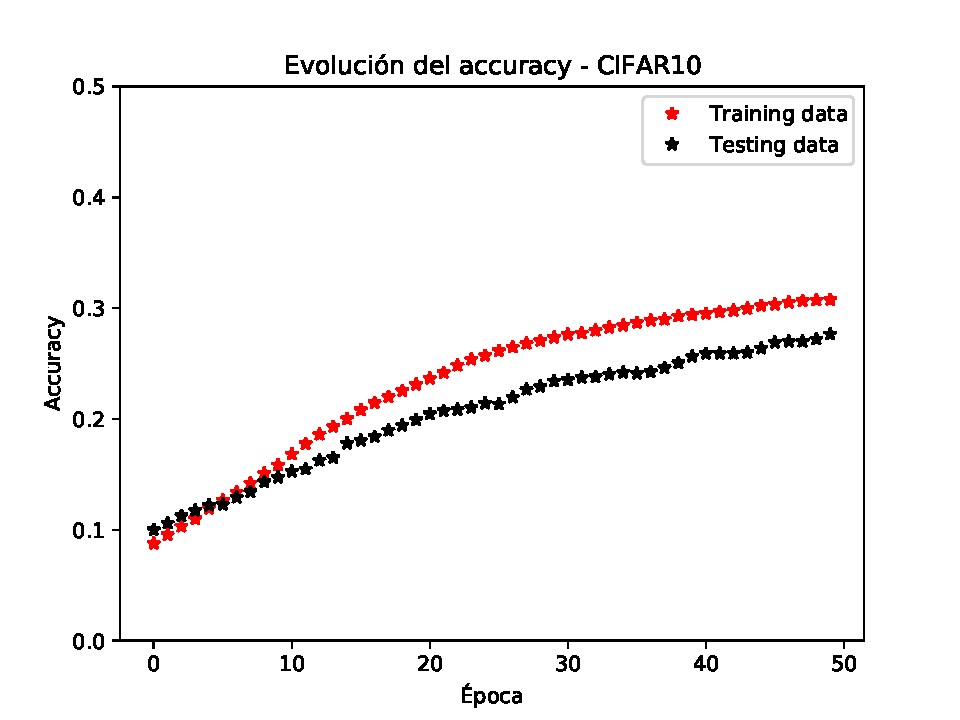
\includegraphics[width=\textwidth]{image/EJ5_Acc_RELU_SIG_MSE.pdf}
         \caption{Accuracy vs. Épocas para los datos de CIFAR-10 utilizando RELU+Sigmoide como funciones de activación y MSE para el cálculo de la Loss}
         \label{fig:acc6a}
     \end{subfigure}
     \hfill
     \begin{subfigure}[b]{0.45\textwidth}
         \centering
         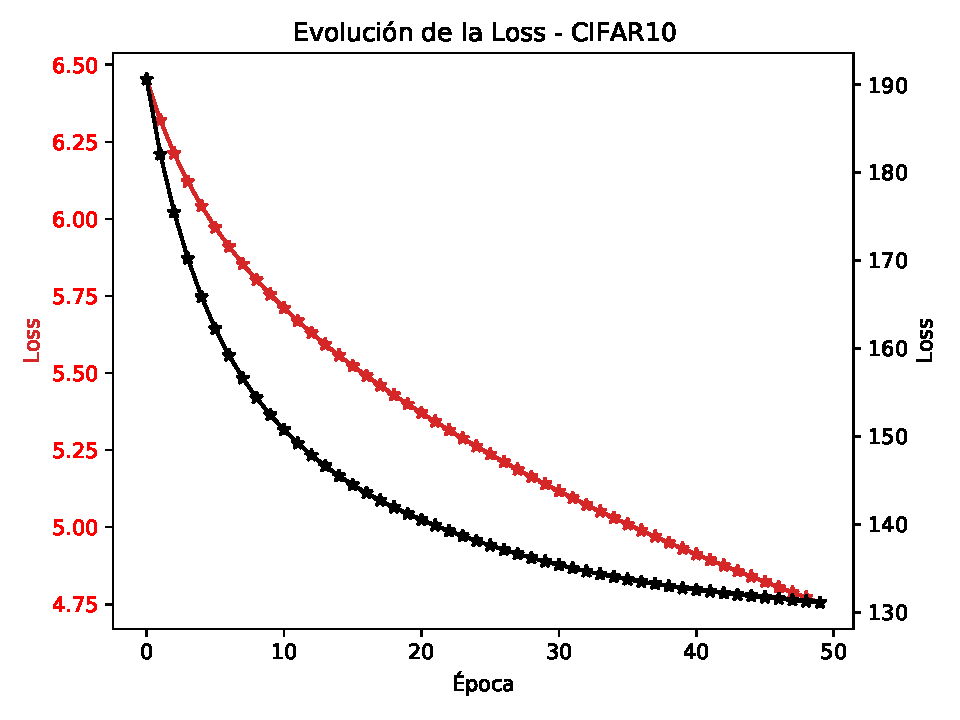
\includegraphics[width=\textwidth]{image/EJ5_Loss_RELU_SIG_MSE.pdf}
         \caption{Loss vs. Épocas para los datos de CIFAR-10 utilizando RELU+Sigmoide como funciones de activación y MSE para el cálculo de la Loss}
         \label{fig:loss6a}
     \end{subfigure}
    \begin{subfigure}[b]{0.45\textwidth}
         \centering
         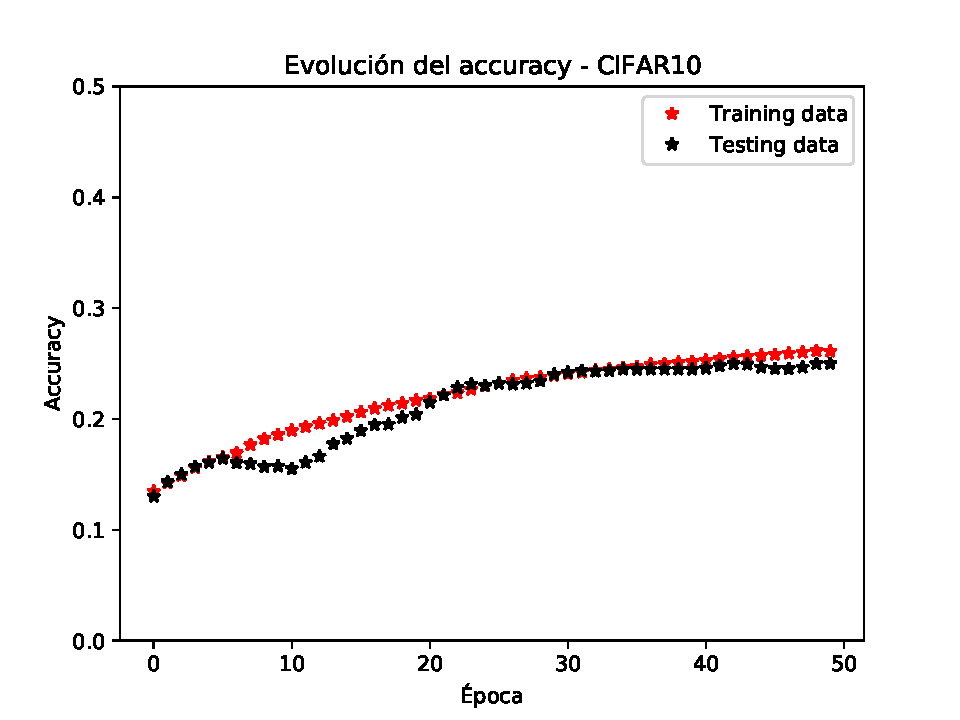
\includegraphics[width=\textwidth]{image/EJ5_Acc_RELU_SIG_SMAX.pdf}
         \caption{Accuracy vs. Épocas para los datos de CIFAR-10 utilizando RELU+Sigmoide como funciones de activación y CCE para el cálculo de la Loss}
         \label{fig:acc6a}
     \end{subfigure}
     \hfill
     \begin{subfigure}[b]{0.45\textwidth}
         \centering
         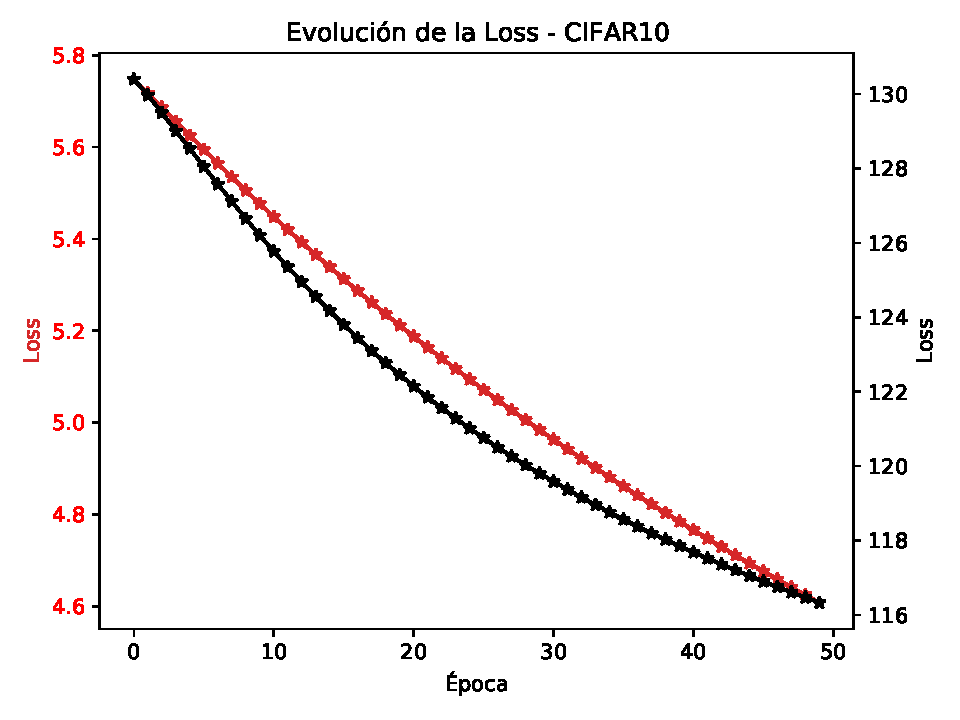
\includegraphics[width=\textwidth]{image/EJ5_Loss_RELU_SIG_SMAX.pdf}
         \caption{Loss vs. Épocas para los datos de CIFAR-10 utilizando RELU+Sigmoide como funciones de activación y CCE para el cálculo de la Loss}
         \label{fig:loss6a}
     \end{subfigure}
        % \caption{Resultados para la segunda arquitectura presentada para resolver el problema de la regla XOR con dos capas densas}
        % \label{fig:resu6a}
\end{figure}

De los resultados obtenidos se ve que para la combinación RELU+Sigmoide como funciones de activación se alcanzó una mejor precisión para la función de costo de MSE, con la cual el accuracy alcanzó 32\% contra un accuracy del 27\% para el CCE.

Si ahora se cambia la función de activación de la segunda capa pos la función lineal (es decir, solo se se hace el producto de las matrices de entrada de la segunda capa con la matriz W2) y para los mismos hiperparámetros se obtienen las siguientes gráficas:



\begin{figure}[H]
     \centering
     \begin{subfigure}[b]{0.45\textwidth}
         \centering
         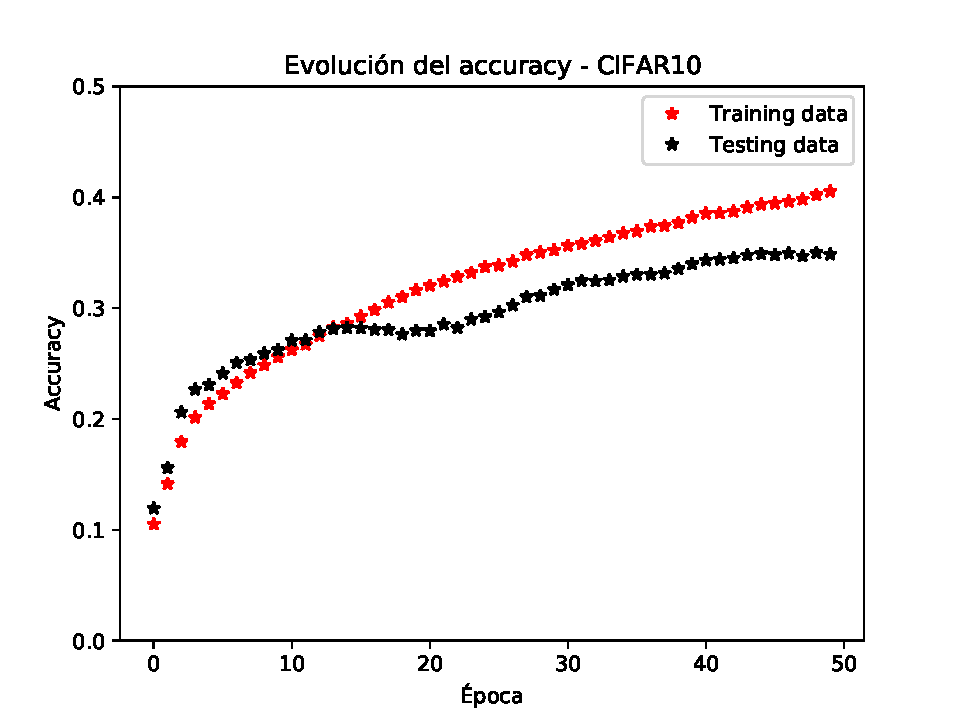
\includegraphics[width=\textwidth]{image/EJ5_Acc_RELU_LIN_MSE.pdf}
         \caption{Accuracy vs. Épocas para los datos de CIFAR-10 utilizando RELU+Lineal como funciones de activación y MSE para el cálculo de la Loss}
         \label{fig:acc6a}
     \end{subfigure}
     \hfill
     \begin{subfigure}[b]{0.45\textwidth}
         \centering
         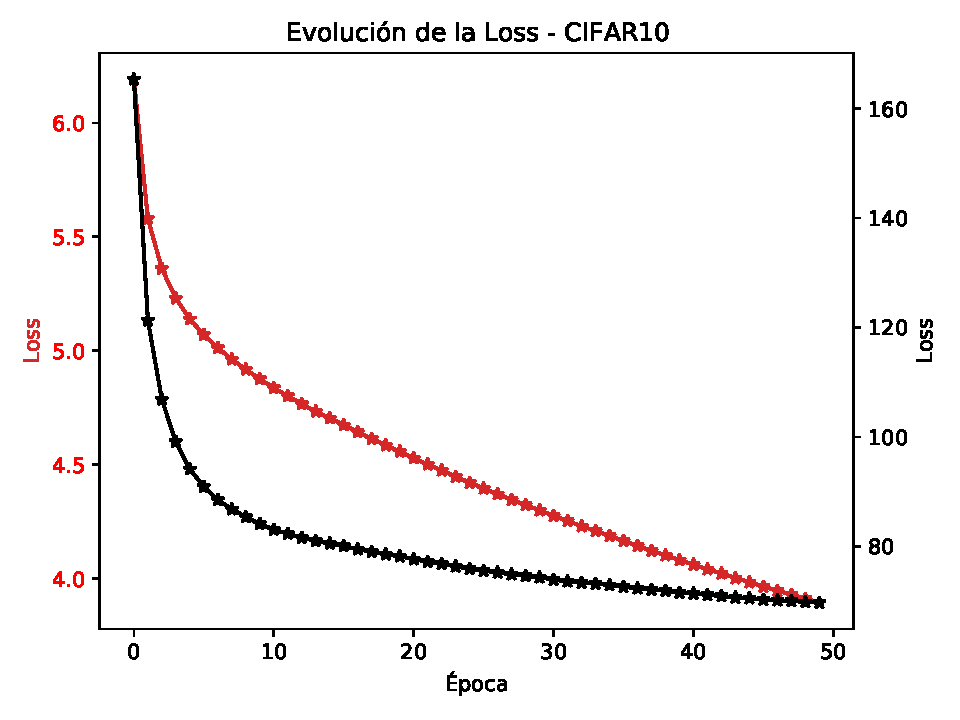
\includegraphics[width=\textwidth]{image/EJ5_Loss_RELU_LIN_MSE.pdf}
         \caption{Loss vs. Épocas para los datos de CIFAR-10 utilizando RELU+Lineal como funciones de activación y MSE para el cálculo de la Loss}
         \label{fig:loss6a}
     \end{subfigure}
    \begin{subfigure}[b]{0.45\textwidth}
         \centering
         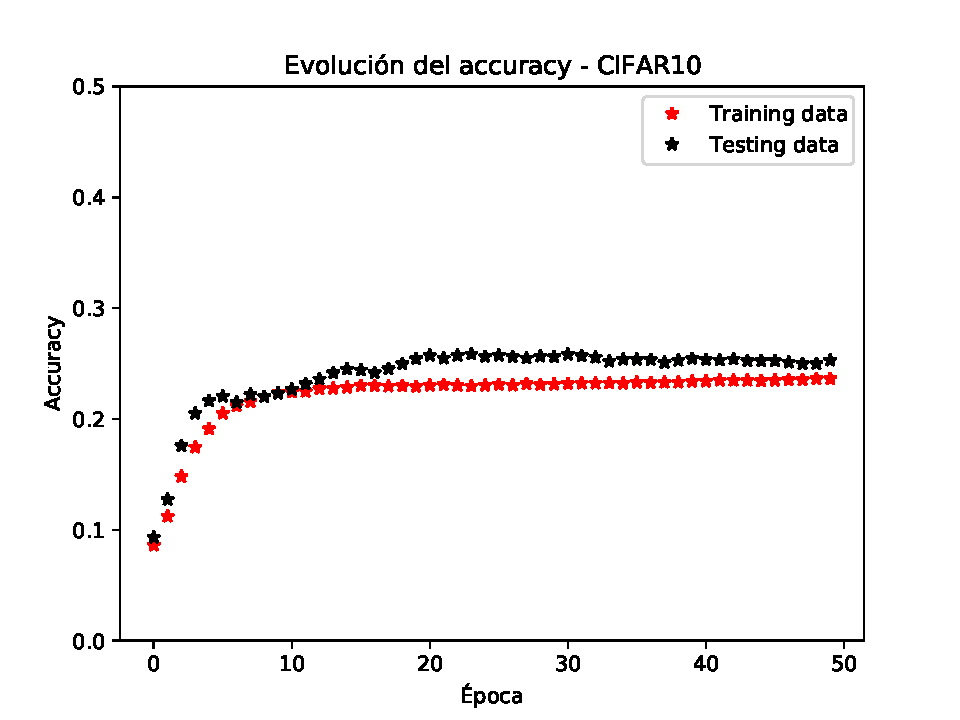
\includegraphics[width=\textwidth]{image/Accuracy50bz128td10000 - RELULIN-SMAX.pdf}
         \caption{Accuracy vs. Épocas para los datos de CIFAR-10 utilizando RELU+Lineal como funciones de activación y CCE para el cálculo de la Loss}
         \label{fig:acc6a}
     \end{subfigure}
     \hfill
     \begin{subfigure}[b]{0.45\textwidth}
         \centering
         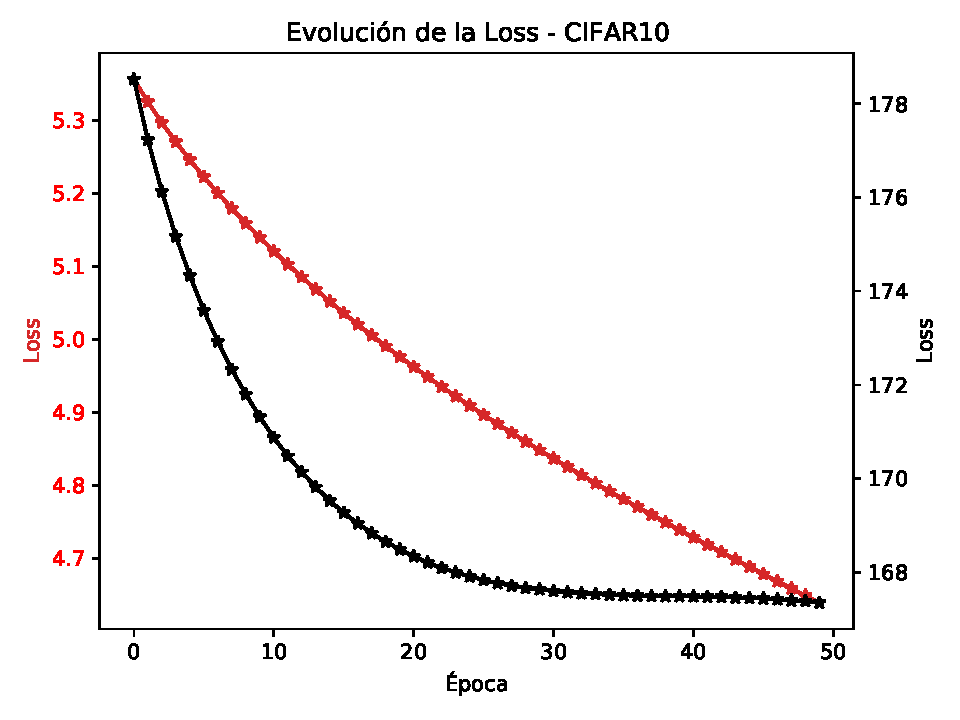
\includegraphics[width=\textwidth]{image/Loss_ep50bz128td10000 - SMAX - RELULIN.pdf}
         \caption{Loss vs. Épocas para los datos de CIFAR-10 utilizando RELU+Lineal como funciones de activación y CCE para el cálculo de la Loss}
         \label{fig:loss6a}
     \end{subfigure}
        % \caption{Resultados para la segunda arquitectura presentada para resolver el problema de la regla XOR con dos capas densas}
        % \label{fig:resu6a}
\end{figure}

De estos resultados se ve que la precisión para ambas la función de costo MSE se alcanza un 35\% y  para la función de costo CCE se logra un 25\% de precisión. 

Analizando los cuatro casos anteriores, se ve que la función de costo MSE es la que consigue una mejor precisión para ambos esquemas de la red (RELU+Sigmoide y RELU+Lineal). En cuanto a si es mejor utilizar la activación Sigmoidal o Lineal para la segunda capa, se podría decir que se obtienen resultados similares para ambas funciones de activación. Sin embargo, debería esperarse que la función de activación Sgimoidal funcione mejor para este problema dado que las etiquetas de cada imagen fue reacondicionada para indicar que si la imagen pertenece a la clase por ejemplo 3, entonces la etiqueta se expresa como 0001000000, es decir, colocando un 1 en la posición correspondiente a la clase de la imagen y 0 en el resto de las clases. Esto tiene relevancia porque como la función Sigmoide toma valores entre 0 y 1, uno esperaría que sea adecuado usar esta función para esta manera de etiquetar los objetos a clasificar. Con la función lineal como activación, la salida podría tomar valores negativos, que para el criterio de clasificación propuesto no tiene sentido un valor negativo. La función lineal debería funcionar mejor para un conjunto de valores no acotados entre 0 y 1. Notar que si el conjunto de valores que puede tomar la salida es mayor que 1 y/o menor que 0, la función de activación sigmoidal tendería a saturar las salidas entre los valores límites 0 y 1.
